\chapter[Planejamento do Projeto]{Planejamento do Projeto}
Neste capítulo será explicado o planejamento utilizado pelo Grupo 1, e justificativas sobre certas decisões.

\section{SAFe}
O SAFe traz tipos de planejamento diferentes para cada nível de projeto. Há o planejamento do épico, o planejamento da \emph{release}, o planejamento da \emph{sprint}, entre outros.

\subsection{Planejamento no Nível de Portfólio}
O planejamento neste nível será baseado no planejamento de um determinado \emph{épico}, organizo pelos \emph{Epic Owners}. Além disso, o gerenciamento neste nível de projeto também será feito pelo \emph{epic owner}.

\subsection{Planejamento no Nível de Programa}
O planejamento no Nível de Programa será baseado no planejamento da \emph{release}, organizada pelo RTE no contexto do grupo 1. Além disso, para ajudar no planejamento, haverá o \emph{Roadmap}, que será atualizado após o \emph{release planning}.

\subsection{Planejamento no Nível de Time}
O planejamento no Nível de Time será baseado no planejamento da \emph{sprint}, organizada pelo Scrum Master, influenciada pelos Desenvolvedores e Product Owners no contexto do grupo 1. Haverá um \emph{kanban} deste nível mostrando entregas a serem feitas, o que está sendo feito, etc. Após as \emph{sprints} ocorrerá a retrospectiva, e seus resultados irão influenciar no planejamento da próxima \emph{sprint}.

\section{Cronograma}
O cronograma ajudará as equipes fornecendo uma visão sobre as tarefas a serem desenvolvidas, o pré-requisito dessas tarefas, e o prazo disponível. Os cronogramas de MPR e Requisitos embora não estejam atrelados entre si, estão conectados de diversas maneiras. Exemplo: certas atividades de Requisitos tem como pré-requisitos atividades de MPR, e este \emph{link} é demonstrado. Certas atividade de Requisitos necessitam ser completadas também por membros de MPR, o que também é demonstrado (designação de tarefa). O cronograma foi feito no \emph{software} Gantter, que se adequou muito bem ao time por ser facilmente gerenciado, ter um bom \emph{track} de ações, ser em nuvem, seguro, entre outras qualidades.

Embora no cronograma pudesse ser especulado possíveis datas para tarefas futuras (exemplo: futuros planejamentos de \emph{release}), tais especulações ainda não são mostradas, pois julga-se como muito cedo. Além disso, são marcados no cronograma marcos importantes do projeto, como por exemplo, o PC, data de entrega do trabalho, entre outros.

Cronograma:

\begin{figure}[h]
  \centering
  \caption{Cronograma da equipe de Requisitos, feito no \emph{Gantter}}
  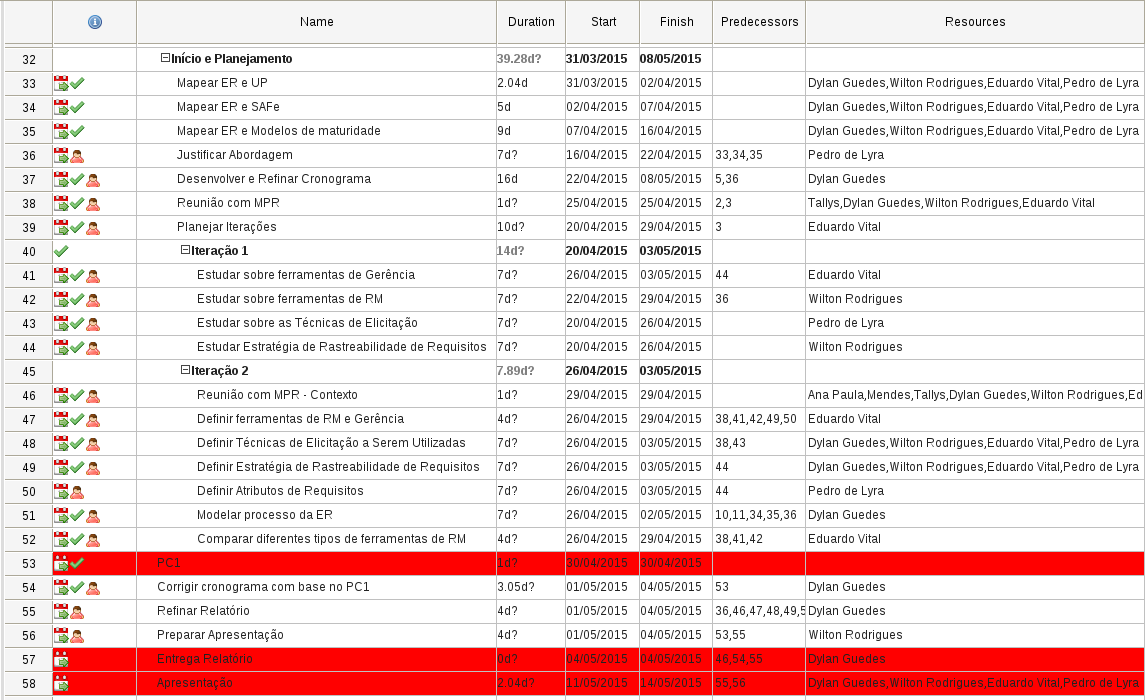
\includegraphics[width=400px, scale=0.5]{figuras/Cronograma001.ps}
\end{figure}

\begin{figure}[h]
  \centering
  \caption{Status das atividades de Requisitos, feito no \emph{Gantter}}
  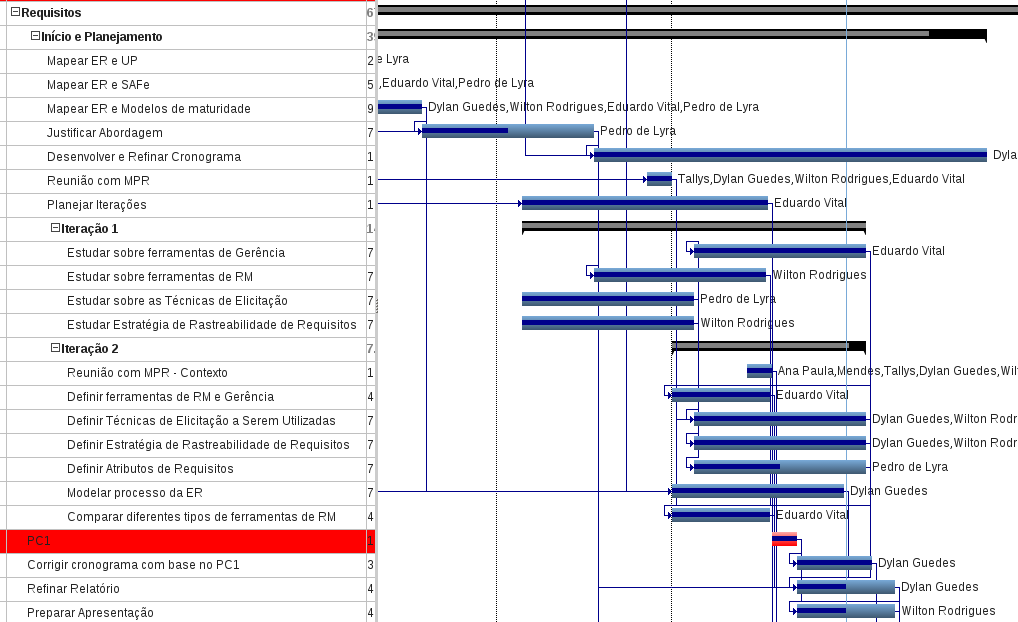
\includegraphics[width=400px, scale=0.5]{figuras/Cronograma002.ps}
\end{figure}

